\section{Methodology} \locallabel{sec:methodology}

\begin{figure}[!t]
\centering \includegraphics[width=3.3in]{graphs/process.eps}
\caption{Visualizes the process of testing and improving the curriculum.}
\locallabel{fig:process}
\end{figure}

\begin{table}
\centering
\begin{tabular}{|c|c|c|c|c|c|} \hline
Class & Grade & Students & Snapshots & Notes & Location \\ \hline \hline
S0A & \nth{4} & 18 & 74 & Yes & Local\\ \hline  % WAF
S0B & \nth{4} & 24 & 94 & Yes & Local\\ \hline  % WABG
S0C & \nth{5} & 39 & 219 & Yes & Local\\ \hline % MH5B
S1A & \nth{4} & 17 & 208 & Yes & Local\\ \hline % MCS
S1B & \nth{4} & 12 & 89 & Yes & Local\\ \hline  % RIOK
S2A & \nth{6} & 31 & 268 & No & Remote\\ \hline % VVSH
S2B & \nth{4} & 20 & 69 & No & Local\\ \hline   % PEASTIRLING
S2C & \nth{4} & 23 & 117 & No & Local\\ \hline  % PEARODRIGUEZ
S2D & \nth{4} & 21 & 67 & No & Local\\ \hline   % PEAGILL
S2E & \nth{4} & 25 & 117 & No & Local\\ \hline  % PEADAHLIN
\end{tabular}
\caption{Participating classes prefixed by assignment iteration (i.e.,
  \emph{S0}, \emph{S1}, or \emph{S2}), with the grade levels represented, the
  number of students with consent, the number of snapshots collected, whether
  field notes were taken, and whether the class was local or remote.}
\locallabel{table:classes}
\end{table}

Our study is informed by design-based research methods and uses both
qualitative and quantitative data and analysis. Design-based research studies
simultaneously inform the development of curriculum, research, and practice,
allowing us to iteratively improve our curriculum as we learn more about
student learning~\cite{barab04,brown92,wang05}. These changes in curriculum in
turn change the learning outcomes. As we are in the initial stages of what will
be both a technological (modified interface) and curricular innovation, we
require a research plan that is able to inform the simultaneous separate but
coordinated development along both technological and curricular
directions. Wang defines design-based research as ``a systematic but flexible
methodology aimed to improve educational practices through iterative analysis,
design, development, and implementation, based on collaboration among
researchers and practitioners in real-world settings, and leading to
contextually-sensitive design principals and theories''~\cite{wang05}.

\subsection{Classes}
\locallabel{sec:classes}
This study involved eight \nth{4} grade, one \nth{5} grade, and one \nth{6}
grade class across California. In all classes we collected snapshots of the
students' work. Additionally, in the first five classes we observed instruction
and interviewed students. Each class had a varying number of students and
snapshots, as well as different start dates. The participating classes are
presented in Table~\localref{table:classes}.

In what we refer to as \emph{wave 0}, classes \emph{S0A}, \emph{S0B}, and
\emph{S0C} piloted the curriculum. This wave was used exclusively to work out
our procedures for collecting data, and curriculum dissemination. The data for
this wave are therefore inconsistent, thus we do not analyze the snapshots and
field notes as part of this study.

All classes, save for \emph{S2A}, were local. Education researchers went to the
local classes to assist in teaching and helping students. The researcher's
presence in the classes as participant observers allowed us to discover
concepts the students were struggling to learn as the researchers wrote field
notes following each visit~\cite{spradley80}. In addition, for all classes, we
automatically generated and captured multiple snapshots of each student's
development process as prior work has found that the final result of student's
development process does not accurately reflect student
understanding~\cite{Piech:2012:MSL:2157136.2157182,brennan12}. The snapshot
generation, collection, and verification process is described in
section~\localref{sub:collection}.

Computer science researchers read the field notes and manually inspected a
subset of student snapshots to discover how the program deviated from what was
intended. This process allowed us to identify features of snapshots that
indicated challenges to students. For example, a snapshot may have unexpected
code-blocks, code-blocks associated with incorrect sprites, or missing
code-blocks.  After we identified those features of snapshots that could
indicate challenges, the entire set of student snapshots was automatically
assessed to quantify the manifestation of each feature. Finally, computer
science and education researchers met to discuss conceptual issues, sources of
those conceptual issues, and changes to make to the lesson, assignment, and
Scratch programming environment. This process was repeated with each subsequent
wave of classes. The entire process is visualized in
Figure~\localref{fig:process}.

\subsection{Our Scratch Interface}
\locallabel{sub:interface}
Prior work by Lewis showed that students using Scratch, aged 10--12, had less
confidence in their response to the statement ``I am good at writing computer
programs'' than students using Logo, a text-based language. Lewis hypothesizes
that the students had not used all the blocks available within Scratch, thus
distorting the students' view of their
abilities~\cite{Lewis:2010:PES:1734263.1734383}. As part of our prior work, we
ran a two week Scratch summer camp where our staff members noted that students
of similar age to those in the camp were often distracted or overwhelmed by the
plethora of blocks available when the assignment only required use of a small
subset of them~\cite{Franklin:2013:SBO}. Furthermore, Halgren et al., reported
that children aged 5--14 have a curiosity to explore available functionality in
their movie-making program:

\begin{quote}Our kids quickly got themselves trapped in
advanced paint and move-making modes which surpassed their expertise. They also
loved clicking on the character buttons at the bottom of the screen. Each click
of a character button placed a new character on the center of the
screen~\cite{Halgren:1995:AAM:223904.223974}.
\end{quote}

While students' curiosity to explore is amazing, it can be a hindrance in the
classroom. Thus, in order to avoid confusion, minimize distraction, and attempt
to maximize students' programming confidence, we applied instructional
scaffolding to Scratch by removing unnecessary blocks. For this assignment, we
removed all but the following blocks:

\begin{itemize}
\item \glideDIST{} (and a variation that adjusted speed)
\item \emph{turn clockwise NUM degrees}
\item \emph{turn counterclockwise NUM degrees}
\item \pointDIR{} (where X is \emph{left}, \emph{right},
  \emph{up} or \emph{down})
\end{itemize}

\subsection{The Sequential Execution Assignment}
\locallabel{sub:sequential_execution}

\begin{figure}[!t]
\centering \includegraphics[width=3.3in]{graphs/screen_s1.eps}
\caption{Initial screen for \sone{} including five sprites. The students task
  was to move the \net{} to \catch{} the \bear{}, the \horse{}, and the
  \zebra{} in any order whilst avoiding the \snake{}. \stwo{} visually differs
  only by the absence of the \snake{}.}
\locallabel{fig:screen_s1}
\end{figure}


\begin{figure}[!t]
\centering 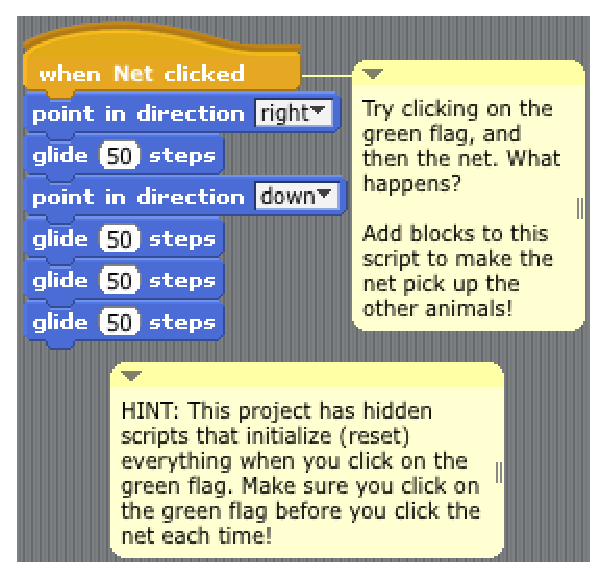
\includegraphics[width=3.3in]{graphs/screen_blocks.eps}
\caption{The script and comments provided in the base project to the students
  in \stwo{}. The script was the same in \sone{}, however, it did not include
  the comments.}
\locallabel{fig:initial_blocks}
\end{figure}


For the purposes of this paper we consider the first assignment given to each
of the three \emph{waves} of classes. The high-level goal of this assignment
was for student to demonstrate a competency in their ability to create a
sequence of instructions in order to accomplish the given task. More
specifically, the goals were for students to

\begin{itemize}
\item have confidence using the interface
\item recognize additional blocks are to be added to the provided base script
\item understand the importance of block ordering within the script
\item understand that execution occurs \netclicked{}
\end{itemize}

While the goals of the assignment in \emph{wave 0} were consistent with those
in the latter waves, the collected snapshots are inconsistent amongst
\emph{wave 0} students. Therefore, we will not discuss that iteration of the
assignment. However, with the latter two waves of classes came two iterations
of the sequential execution project that we will discuss: \sone{} and \stwo{}.

\subsubsection{Iteration 1: \sone{}}
\locallabel{sub:s1}
The first iteration of the sequential execution assignment, referred to as
\sone{}, presents students with the \stage{} and five sprites arranged as shown
in Figure~\localref{fig:screen_s1}. In the sequential execution assignment the
students are to program the navigation for the \net{}, located in the upper
left, such that it \catch{es} the \bear{}, located in the upper right, the
\horse{}, located in the middle right, and the \zebra{}, located in the lower
left. The students are permitted to program the \net{} to \catch{} these
sprites in any order they desire. However, in \sone{}, the students are
presented with an obstacle to avoid, the \snake{}, located in the lower right.

The students were provided with a base project that moved the \net{} such that
it \caught{} the \zebra{} using a combination of \glideDIST{} and \emph{point
  in direction X} blocks as depicted in
Figure~\localref{fig:initial_blocks}. In section~\localref{sub:approach} we
classify this combination of blocks as an \textbf{orient and glide} approach
utilizing \textbf{absolute} orientation.

\subsubsection{Iteration 2: \stwo{}}
The second iteration, referred to as \stwo{}, presents students with a screen
similar to that in Figure~\localref{fig:screen_s1}. The only visual difference
is the removal of the \snake{}. Aside from needing to avoid the \snake{}, both
the students' objective and provided base project remained the same. However,
in addition to the blocks included in \sone{}, we added two other block
choices:

\begin{itemize}
\item \pointtoward{}
\item \glideto{}
\end{itemize}

The \glideto{} block is a custom block we added to Scratch after observing
student difficultly during \sone{} with the two blocks required to successfully
move the \net{}. Despite the addition of \glideto{}, the students were not
prompted to use it. A comparison of student block choices is provided in
section~\localref{sub:approach}. One other notable change made to the Scratch
interface for \stwo{} was the removal of the \dce{} functionality provided by
Scratch. See section~\localref{sub:dce} for a discussion of why we removed this
functionality.

\subsection{Capturing, Collecting, and Verifying the Accuracy of Snapshot Generation}
\locallabel{sub:collection}
Scratch, like many computer programs, only saves the most recent version of
work when explicitly directed to do so through a \emph{save} action. In order
to possess snapshots of students' in-progress work, we modified Scratch to
automatically generate a snapshot when two conditions are met: the \emph{green
  flag} button is clicked, and at least four modifications to the student's
program have occurred since the last snapshot. We consider clicking the
\emph{green flag} to be a unit of work, because that is how students test their
program. Snapshots are also created whenever the student explicitly invokes the
\emph{save} action. All snapshots for a student are timestamped and combined in
one zip archive to reduce both the size and number of files we needed to
collect.

We did not create a snapshot on every \emph{green flag} button click due to a
network issue we experienced during teacher training. The computers we trained
the teachers on were configured such that Scratch save files were actually
stored on a remote server, thus each save required transferring data over the
network. While the creation of a single snapshot is not an issue, the
concurrent creation of many is. Because many school networks are configured
similarly, we introduced the four modification snapshot creation condition in
hopes of preventing this network issue; it worked.

Students were asked to submit their single snapshot archive at the end of each
work period by uploading the file through a web service we wrote for collection
purposes. This web service associated each student with their uploaded
snapshots. While this process was very effective, and much less error prone
than the researchers manually fetching files from computers, it was not without
issue; there were three:

\begin{enumerate}
\item A few students accidentally submitted the work of a student who had used
  the same computer in a previous class due to the web browser's recall of the
  directory of the last uploaded file.
\item Instead of starting with the provided base-project, a few students
  accidentally started with a snapshot of a student who had used the same
  computer in a previous class.
\item Some students submitted only the final version of their work due to
  selecting the final version file rather than the snapshot archive file.
\end{enumerate}

Fortunately, we were able to utilize the save-log contained within each Scratch
save-file (i.e., our snapshots) to identify students who experienced any of
these three issues, and for issue \#1 we were able to retroactively obtain the
snapshots for some of the affected students. The save-log in a Scratch
save-file records the history of every \emph{save} action with a timestamp and
the name of the file saved to. From this information we identified students
sharing unexpected common starting points. That is, students who share more
than one consecutive entry in their files' save-logs that immediately succeeds
the save-log of the file we provided the students to start with. Once
identified, we disassociated these snapshots from the student in the
chronologically later class. This procedure was used to resolve issues \#1 and
\#2. We resolved issue \#3 by comparing the number of snapshots collected for a
student to the number of snapshots captured as recorded in the
save-log. Students with fewer snapshots than expected were removed from our
dataset. Because we did not analyze any of the \emph{wave 0} classes, we also
did not validate the data for those classes. Thus the \emph{student} and
\emph{snapshot} values for the first three columns in
Table~\localref{table:classes} are an upper bound.
